\RequirePackage{fix-cm}
\documentclass{bmstu-sob}

% ------------------------------------------------------------
% Латиница
% ------------------------------------------------------------
% bmstu-sob использует XeLaTeX/LuaLaTeX и сам настраивает
% основной шрифт. Поэтому fontspec здесь повторно не подключаем.
%
% Латинские идентификаторы SQL:
% users, wallets, operations, operation_types
% поддерживаются непосредственно.

% ------------------------------------------------------------
% Нумерация разделов без привязки к главам
% ------------------------------------------------------------
\renewcommand{\thesection}{\arabic{section}}
\renewcommand{\thesubsection}{\arabic{section}.\arabic{subsection}}

% ------------------------------------------------------------
% Документ
% ------------------------------------------------------------
\begin{document}

% ------------------------------------------------------------
% Титульный лист
% ------------------------------------------------------------
\makereporttitle
    {Платформенные решения для интеллектуального анализа больших данных}
    {Компьютерные системы и сети}
    {лабораторной работе №~1}
    {Технология параллельных систем баз данных}
    {Установка и настройка СУБД PostgreSQL}
    {2}
    {Соболев~Н.~А./ИУ6-13М}
    {Григорьев~Ю.~А.}

\newpage
% ============================================================
% 1. ЦЕЛЬ РАБОТЫ
% ============================================================

\section{Цель работы}

Целью лабораторной работы является формирование следующей
компетенции: студент должен получить навыки инсталляции СУБД
PostgreSQL в среде ОС Ubuntu, протестировать её работу,
разработать небольшую базу данных и выполнить запросы к ней.

% ============================================================
% 2. СОЗДАНИЕ ТАБЛИЦЫ users
% ============================================================

\section{Создание таблицы users}

Создана последовательность \texttt{user\_ids} и таблица
\texttt{users}:

\begin{lstlisting}[language=SQL]
CREATE SEQUENCE user_ids;

CREATE TABLE users (
    id INTEGER PRIMARY KEY DEFAULT nextval('user_ids'),
    surname VARCHAR(64),
    firstname VARCHAR(64)
);
\end{lstlisting}

Добавлены записи:

\begin{lstlisting}[language=SQL]
INSERT INTO users (surname, firstname)
VALUES ('Иванов', 'Иван');

INSERT INTO users (surname, firstname)
VALUES ('Петров', 'Пётр');
\end{lstlisting}

Выполнен поиск:

\begin{lstlisting}[language=SQL]
SELECT * FROM users;

SELECT *
FROM users
WHERE surname = 'Иванов';
\end{lstlisting}

Результат представлен на рисунке~\ref{fig:query}.

\begin{figure}[htbp]
    \centering
    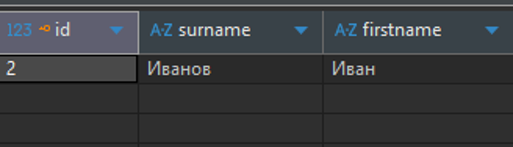
\includegraphics[
        width=0.6\textwidth
    ]{img/результат_запроса.png}
    \caption{Результат запроса}
    \label{fig:query}
\end{figure}

% ============================================================
% 3. ВАРИАНТ 2. СЕРВИС «КОШЕЛЁК»
% ============================================================

\section{Вариант 2. Сервис «кошелёк»}

\subsection{Схема базы данных}

Для реализации сервиса «кошелёк» используются таблицы
\texttt{users}, \texttt{wallets}, \texttt{operations} и
\texttt{operation\_types}.

Таблица \texttt{users} содержит сведения о пользователях.
Таблица \texttt{wallets} содержит сведения о кошельках
пользователей. Таблица \texttt{operation\_types} предназначена
для хранения типов операций, а таблица \texttt{operations}
содержит сведения о выполненных операциях.

Схема базы данных представлена на рисунке~\ref{fig:schema}.

\begin{figure}[htbp]
    \centering
    
\includegraphics[
        width=0.8\textwidth
    ]{img/схема_бд.png}
    \caption{Схема базы данных}
    \label{fig:schema}
\end{figure}

\subsection{Создание таблиц}

Таблица \texttt{wallets} создаётся следующим запросом:

\begin{lstlisting}[language=SQL]
CREATE TABLE wallets (
    id INTEGER PRIMARY KEY,
    user_id INTEGER NOT NULL,
    currency VARCHAR(3) NOT NULL,
    CONSTRAINT fk_wallet_user
        FOREIGN KEY (user_id)
        REFERENCES users(id)
);
\end{lstlisting}

Таблица \texttt{operation\_types} создаётся следующим запросом:

\begin{lstlisting}[language=SQL]
CREATE TABLE operation_types (
    id INTEGER PRIMARY KEY,
    name VARCHAR(64) NOT NULL
);
\end{lstlisting}

Таблица \texttt{operations} создаётся следующим запросом:

\begin{lstlisting}[language=SQL]
CREATE TABLE operations (
    id INTEGER PRIMARY KEY,
    wallet_id INTEGER NOT NULL,
    operation_type_id INTEGER NOT NULL,
    amount NUMERIC(12, 2) NOT NULL,
    operation_date TIMESTAMP NOT NULL,

    CONSTRAINT fk_operation_wallet
        FOREIGN KEY (wallet_id)
        REFERENCES wallets(id),

    CONSTRAINT fk_operation_type
        FOREIGN KEY (operation_type_id)
        REFERENCES operation_types(id)
);
\end{lstlisting}

% ============================================================
% 4. ЗАПРОС
% ============================================================

\subsection{Запрос}

Для получения информации об операциях пользователя выполнен
следующий SQL-запрос:

\begin{lstlisting}[language=SQL]
SELECT
    u.surname,
    u.firstname,
    u.city,
    w.currency,
    o.amount,
    o.operation_date,
    ot.name AS operation_type
FROM users u
JOIN wallets w
    ON w.user_id = u.id
JOIN operations o
    ON o.wallet_id = w.id
JOIN operation_types ot
    ON ot.id = o.operation_type_id
WHERE u.surname = 'Иванов'
  AND u.city = 'Москва'
  AND w.currency = 'USD'
  AND ot.name = 'Снятие'
  AND o.operation_date >= '2020-01-01'
  AND o.operation_date < '2020-09-02'
ORDER BY o.operation_date;
\end{lstlisting}

Результат представлен на рисунке~\ref{fig:result}.

\begin{figure}[htbp]
    \centering
    
\includegraphics[
        width=\textwidth
    ]{img/результат_запроса2.png}
    \caption{Результат запроса}
    \label{fig:result}
\end{figure}

% ============================================================
% 5. ВЫВОД
% ============================================================

\section{Вывод}

В ходе лабораторной работы были получены навыки установки СУБД
PostgreSQL в ОС Ubuntu, проверки её работоспособности, разработки
базы данных и выполнения запросов.

Разработана база данных для сервиса «кошелёк», включающая таблицы
\texttt{users}, \texttt{wallets}, \texttt{operations} и
\texttt{operation\_types}. Выполнен запрос с соединением четырёх
таблиц и фильтрацией по нескольким условиям.

\end{document}